\documentclass[a4paper,11pt,fleqn,dvipsnames,twoside,openright]{memoir} 	

%%%% PACKAGES %%%%
% ¤¤ Encoding and language ¤¤ %
\usepackage[utf8x]{inputenc}				
\usepackage[UKenglish]{babel}				
\usepackage[T1]{fontenc}				
\usepackage{ragged2e,anyfontsize}		
\usepackage{fixltx2e}

% ¤¤ Figures and tables (floats) ¤¤ %
\usepackage{graphicx} 					
\usepackage{multirow}                
\usepackage{multicol}         	       
\usepackage{rotating}					
\usepackage{colortbl} 					
\usepackage[table]{xcolor}						
\usepackage{flafter}					
\let\newfloat\relax 					
\usepackage{float}		
\usepackage{longtable}	
\usepackage{etoolbox}
\usepackage{placeins}

% ¤¤ Math ¤¤ %
\usepackage{amsmath,amssymb,stmaryrd} 	
\usepackage{mathtools}					
\usepackage{textcomp}                 	
\usepackage{rsphrase}				
\usepackage[version=3]{mhchem} 			
\usepackage{siunitx}					

% ¤¤ References and sources ¤¤ %
\usepackage[english]{varioref}			
\usepackage{natbib}              			

% ¤¤ Misc. ¤¤ %
\usepackage{listings}
\usepackage{color}
\usepackage{courier}
\usepackage{dirtree}
%\usepackage{lipsum}						
\usepackage[shortlabels]{enumitem}		
\usepackage{pdfpages}	
\usepackage{mdframed}
\pdfoptionpdfminorversion=6				
\pretolerance=2500


\usepackage[footnote,draft,english,silent,nomargin]{fixme}		
\usepackage{lastpage}

%%%% CUSTOM SETTINGS %%%%
% ¤¤ Margins ¤¤ %
\setlrmarginsandblock{3.5cm}{2.5cm}{*}	
\setulmarginsandblock{2.5cm}{3.0cm}{*}	
\checkandfixthelayout 					

% ¤¤ Formatting ¤¤ %
\setlength{\parindent}{0mm}           	
\setlength{\parskip}{3mm}          		
\linespread{1,1}					

% ¤¤ Literature list ¤¤ %
\bibpunct[,]{[}{]}{;}{a}{,}{,} 
\bibliographystyle{plainnat}	

% ¤¤ Table of contents ¤¤ %
\setsecnumdepth{subsection}		 		
\maxsecnumdepth{subsection}				
\settocdepth{section} 				

% ¤¤ Lists ¤¤ %
\setlist{
  topsep=0pt,							
  itemsep=-1ex,							
} 

\newcommand*\Hide{%
\titleformat{\chapter}[display]
  {}{}{0pt}{\Huge}
\titleformat{\part}
  {}{}{0pt}{}
}

% Chapter med subtitle
\newcommand\Chapter[2]{
  \chapter[#1: {\itshape#2}]{#1\\\Large\itshape#2}
}

% ¤¤ Visual references ¤¤ %
\usepackage[colorlinks]{hyperref}		
\hypersetup{colorlinks = true,	
    linkcolor = black,
    citecolor = black,
    urlcolor = black
}

% ¤¤ Caption layout ¤¤ %
\captionnamefont{\small\bfseries\itshape}	
\captiontitlefont{\small}				
\captiondelim{. }						
\hangcaption							
\captionwidth{\linewidth}				
\setlength{\belowcaptionskip}{0pt}		
		
% ¤¤ Listings layout ¤¤ %
\definecolor{commentGreen}{RGB}{0,150,0}
\definecolor{darkRed}{RGB}{150,0,0}
\definecolor{stringPurple}{RGB}{208,76,239}
\definecolor{light-gray}{gray}{0.95}

\usepackage{caption}
\usepackage{subcaption}
\DeclareCaptionFont{white}{\color{white}}
\DeclareCaptionFormat{listing}{\colorbox{gray}{\parbox{\textwidth-6pt}{#1#2#3}}}
\captionsetup[lstlisting]{format=listing,labelfont=white,textfont=white}



\lstset{
    language=C++,
    basicstyle=\ttfamily\small,
    numbers=left,
    %stepnumber=2,
    numbersep=5pt,
    tabsize=3,
    extendedchars=true,
    breaklines=true,
    keywordstyle=\color{blue}\ttfamily,
    commentstyle=\color{commentGreen}\ttfamily,
    frame=b,
    stringstyle=\color{darkRed}\ttfamily,
    xleftmargin=17pt,
    framexleftmargin=17pt,
    framexrightmargin=5pt,
    framexbottommargin=4pt,
    backgroundcolor=\color{light-gray},
    showstringspaces=false,
    xleftmargin=23pt,
    framexleftmargin=23pt,
    framexrightmargin=0pt,
    framexbottommargin=4pt
 }

% Alternative Listing style (Caption below)
%\lstset{
%    frame=single,
%    tabsize=3,
%    breaklines=true,
%    backgroundcolor=\color{light-gray},
%    language=C++,
%    basicstyle=\ttfamily,
%    keywordstyle=\color{blue}\ttfamily,
%    stringstyle=\color{red}\ttfamily,
%    commentstyle=\color{commentGreen}\ttfamily,
%    belowcaptionskip=4pt,
%    captionpos=b,
%    numbers=left,
%    morecomment=[l][\color{magenta}]{\#}
%}




		
% ¤¤ Naming ¤¤ %
\addto\captionsenglish{
	\renewcommand\contentsname{Table of contents}	
	\renewcommand\cftchaptername{\chaptername~}			
	\renewcommand\cftappendixname{\appendixname~}		
}

% ¤¤ Chapter layout ¤¤ %
\definecolor{numbercolor}{gray}{0.7}	
\newif\ifchapternonum

\makechapterstyle{jenor}{			
  \renewcommand\beforechapskip{0pt}
  \renewcommand\printchaptername{}
  \renewcommand\printchapternum{}
  \renewcommand\printchapternonum{\chapternonumtrue}
  \renewcommand\chaptitlefont{\fontfamily{pbk}\fontseries{db}\fontshape{n}\fontsize{25}{35}\selectfont\raggedleft}
  \renewcommand\chapnumfont{\fontfamily{pbk}\fontseries{m}\fontshape{n}\fontsize{1in}{0in}\selectfont\color{numbercolor}}
  \renewcommand\printchaptertitle[1]{%
    \noindent
    \ifchapternonum
    \begin{tabularx}{\textwidth}{X}
    {\let\\\newline\chaptitlefont ##1\par} 
    \end{tabularx}
    \par\vskip-2.5mm\hrule
    \else
    \begin{tabularx}{\textwidth}{Xl}
    {\parbox[b]{\linewidth}{\chaptitlefont ##1}} & \raisebox{-15pt}{\chapnumfont \thechapter}
    \end{tabularx}
    \par\vskip2mm\hrule
    \fi
  }
}				

\newfloat{Code}{H}{myc}

\chapterstyle{jenor}			

% ¤¤ Header/footer layout ¤¤ %
\makepagestyle{AAU}						
\makepsmarks{AAU}{%
	\createmark{chapter}{left}{shownumber}{}{. \ }
	\createmark{section}{right}{shownumber}{}{. \ }
	\createplainmark{toc}{both}{\contentsname}
	\createplainmark{lof}{both}{\listfigurename}
	\createplainmark{lot}{both}{\listtablename}
	\createplainmark{bib}{both}{\bibname}
	\createplainmark{index}{both}{\indexname}
	\createplainmark{glossary}{both}{\glossaryname}
}
\nouppercaseheads			

\makeevenhead{AAU}{Group SW606F15}{}{\leftmark}			
\makeoddhead{AAU}{\rightmark}{}{Aalborg University}	
\makeevenfoot{AAU}{\thepage}{}{}						
\makeoddfoot{AAU}{}{}{\thepage}							
\makeheadrule{AAU}{\textwidth}{0.5pt}					
\makefootrule{AAU}{\textwidth}{0.5pt}{1mm}				

\copypagestyle{AAUchap}{AAU}							
\makeoddhead{AAUchap}{}{}{}
\makeevenhead{AAUchap}{}{}{}
\makeheadrule{AAUchap}{\textwidth}{0pt}
\aliaspagestyle{chapter}{AAUchap}							

\pagestyle{AAU}											


%%%% CUSTOM COMMANDS %%%%

% ¤¤ Project name ¤¤
% Skrives som \projname{}
\newcommand{\giraf}{\emph{GIRAF}}

% ¤¤ Referencer ¤¤
\newcommand{\secref}[1]{Section~\ref{#1}}
\newcommand{\charef}[1]{Chapter~\ref{#1}}
\newcommand{\figref}[1]{Figure~\ref{#1}}
\newcommand{\tblref}[1]{Table~\ref{#1}}
\newcommand{\lstref}[1]{Listing~\ref{#1}}
\newcommand{\appref}[1]{Appendix~\ref{#1}}
\newcommand{\equref}[1]{Equation~\ref{#1}}

% ¤¤ Figure hack ¤¤ %
\newcommand{\fig}[4]{
		\begin{figure}[H] \centering
		\includegraphics[width=#1\textwidth]{pictures/#2}
			\caption{#3}\label{#4}
		\end{figure} 
}

% ¤¤ Special characters ¤¤ 
\newcommand{\decC}{^{\circ}\text{C}}
\newcommand{\dec}{^{\circ}}
\newcommand{\m}{\cdot}


%%%% HYPHENATION %%%%
\hyphenation{}


%%%% Noget vi har skrevet/Egne tilføjelser %%%%
\newcommand{\ra}[1]{\renewcommand{\arraystretch}{#1}}
\selectlanguage{UKenglish}
\definecolor{Gray}{gray}{0.92}
\definecolor{DGray}{gray}{0.83}
\definecolor{DarkGray}{gray}{0.35}
\definecolor{mygreen}{rgb}{0,0.6,0}
\usepackage{pxfonts}

%%%% OK lækker kode som fixer vores liv. Dødstaf for at slette det! %%%%
\makeatletter
\pretocmd\start@align
{%
  \let\everycr\CT@everycr
  \CT@start
}{}{}
\apptocmd{\endalign}{\CT@end}{}{}
\makeatother


\makeatletter
\renewcommand\part{%
  \if@openright
    \cleardoublepage
  \else
    \clearpage
  \fi
  \thispagestyle{empty}%   % Original »plain« replaced by »emptyx
  \if@twocolumn
    \onecolumn
    \@tempswatrue
  \else
    \@tempswafalse
  \fi
  \null\vfil
  \secdef\@part\@spart}
\makeatother

%%%% Listing! %%%%

\newenvironment{narrow}[2]{%
  \begin{list}{}{%
    \setlength{\topsep}{0pt}%
    \setlength{\leftmargin}{#1}%
    \setlength{\rightmargin}{#2}%
    \setlength{\listparindent}{\parindent}%
    \setlength{\itemindent}{\parindent}%
    \setlength{\parsep}{\parskip}%
  }%
  \item[]
}{\end{list}}



\definecolor{pblue}{rgb}{0.13,0.13,1}
\definecolor{pgreen}{rgb}{0,0.5,0}
\definecolor{pred}{rgb}{0.9,0,0}
\definecolor{pgrey}{rgb}{0.46,0.45,0.48}

\newcommand{\BigO}[1]{\ensuremath{\operatorname{O}\bigl(#1\bigr)}}
\newcommand{\READ}[1]{\fxnote{\textbf{READV2 #1}}}

\raggedbottom

\begin{document}
\selectlanguage{UKenglish}

\frontmatter							

\thispagestyle{empty}
\begin{flushright}
\vspace{3cm}

\phantom{hul}

\phantom{hul}

\phantom{hul}

\textsl{\Huge Web Service} \\ 


\rule{14cm}{2mm} \\ 
\Huge INTERNET TECHNOLOGY\\ \vspace{1.5cm}

\begin{figure}[H]
     \center{
\includegraphics[width=\textwidth-90px]
     {graphics/Stupid_FP.jpg}}
\end{figure}
% Fix så det passer med nuværende semester og projekt
\vspace{2cm} 
\textsc{\Large Software P7 Project \\
Group SW707E15 \\
Aalborg University\\
Autumn semester 2015\\}
\end{flushright}
\cleardoublepage							
\phantomsection
\pdfbookmark[0]{Titlepage}{titlepage}
\thispagestyle{empty}


\begin{minipage}[t]{0.48\textwidth}
\vspace*{-25pt}

\includegraphics[height=4cm]{graphics/AAU-logo-stud-UK-RGB} 
\end{minipage}
\hfill
\begin{minipage}[t]{0.48\textwidth}
{\small 
\textbf{Department of Computer Science}\\
Aalborg University  \\
Software \\
Selma Lagerl\"{o}fs Vej 300 \\
9220 Aalborg Øst} \\
\url{www.cs.aau.dk}
\end{minipage}

\vspace*{1cm}

\begin{minipage}[t]{0.48\textwidth}
\textbf{Title:} \\[5pt]\bigskip\hspace{2ex}
Project title\\
\textbf{Theme:} \\[5pt]\bigskip\hspace{2ex}
\parbox{6.6 cm}{
Internet technology}

\textbf{Project:} \\[5pt]\bigskip\hspace{2ex}
7th semester

\textbf{Project period:} \\[5pt]\bigskip\hspace{2ex}
September 2015 - December 2015

\textbf{Project group:} \\[5pt]\bigskip\hspace{2ex}
SW707E15

\textbf{Participants:} \\[5pt]\hspace*{2ex}
Jacob Elefsen \\\hspace*{2ex}
Lars Emil Eriksen \\\hspace*{2ex}
Mikkel Giedsing Nielsen \\\hspace*{2ex}
Joakim Iversen \\\hspace*{2ex}
Emil Nesgaard \\\hspace*{2ex}
Tobias Hvass Mølbak \\\bigskip\hspace{2ex}

\textbf{Supervisor:} \\[5pt]\hspace*{2ex}
Hans Hüttel
\vspace*{1cm}

\textbf{Editions: } \\
\textbf{Report pages: \pageref{LastPage}} \\
\textbf{Appendix pages: } \\
\textbf{Completed: }

\end{minipage}
\hfill
\begin{minipage}[t]{0.48\textwidth}
Abstract: \\[5pt]
\fbox{\parbox{7cm}{\bigskipThis project is gonna develop stuff using other existing stuff, all the while writing some stuff about how the stuff was developed. \bigskip}}
\end{minipage}

\vfill

{\footnotesize\itshape The content of the report is freely available, but publication (with source reference) may only take place in agreement with the authors.}


\cleardoublepage
\chapter*{Preface}
This report is written by a group of 7th semester software students at Aalborg University. Throughout the report appropriate terminology is used, this means that the readers must have some knowledge about computer science, more specifically about internet technologies.

The report uses Harvard citation, that provides the name of the author(s) of the source. As an example, the book used in the course Machine Intelligence, is shown as \fxnote{Skift eksempel til et passende} %~\citep{} .

\vspace{25mm}

\noindent\begin{tabular}{ll}
%\includegraphics[width=2.5in]
%{Pictures/jacobelefsen.pdf} &  \\
\makebox[2.5in]{\hrulefill} & \makebox[2.5in]{\hrulefill}\\
Jacob Elefsen & Lars Emil Eriksen\\[8ex]% adds space between the two sets of signatures
\makebox[2.5in]{\hrulefill} & \makebox[2.5in]{\hrulefill}\\
Mikkel Giedsing Nielsen & Joakim Iversen\\[8ex]
\makebox[2.5in]{\hrulefill} & \makebox[2.5in]{\hrulefill}\\
Emil Nesgaard & Tobias Hvass Mølbak
\end{tabular}

\cleardoublepage

%%%% Indholdsfortegnelse (TOC) %%%%
\phantomsection
\pdfbookmark[0]{Table of Contents}{contents}
\tableofcontents*

\mainmatter

%%%% Chapters %%%%
% Dette dokument skal ikke indeholde nogen form for tekst!
% Det er en samling af alle kapitlerne.

% Introduction
\chapter{Introduction} \label{cha:introduction}



% Analysis
\chapter{Analysis} \label{cha:analysis}

A \textit{Smart Home} is a concept of connecting various devices, such as lighting, televisions, and other electronics, providing a common \phone. In recent years having a Smart Home has become increasingly popular, as technology that enables the concept becomes increasingly available for consumers. Numerous companies are trying to establish a foothold in the market, each with their own solution of a Smart Home, for a good reason. Being able to establish a recognisable brand in this market could ensure a bright future, according to statistics. By the end of 2012, 3.5 million Smart Home systems were installed in North America. Since then the number of installations has increased to 13 million in 2015, and by the end of 2017 it has been estimated that 31 million North American homes will have a Smart Home system installed~\citep{statista-na-estimation}.

To ensure less confusion, the following list explains the common key-words that is used within the scope of home automation.
\begin{description}
\item[Smart Home] is used for the concept in its entirety, which includes all of the \sdevs, the \hub, and the \phone~within the same home.
\item[\Hub] commonly used in a Smart Home. All the \sdevs~are connected to it, which allows the users to control their \sdevs~through one application.
\item[\SDevs] are accessible devices and gadgets that can be connected to the Internet, either through a \hub~or directly through the router.
\item[\Phone] is used to administrate the \sdevs. Which can be displayed on any device such as, phone, tablet, or computer application.
\end{description}


% Problem Description
 \section{Problem Setting} \label{sec:problem-description}
There are several different conveniences a Smart Home system could provide, e.g. being able to dim, or turn off the lights while sitting down.
Some Smart Home systems incorporate cameras, which provides the ability to monitor ones home while being away.
The functionality affects various aspects e.g., security, chores, ease-of-life enhancements, and entertainment.

\subsection{Use Cases}\label{sec:use-cases}
The following use cases explain some of the problems that users of Smart Home solutions may encounter:

\begin{colbox}{Use case: John}
John is enthusiastic about gadgets and new technology. He therefore owns a lot of \sdevs~from various manufacturers, and majority of his electronics are connected to the Internet. John wants to put on a movie, turn on his surround sound, and dim the light. To do so he has to find and open the phone application for the television to turn it on. Next he has to find another application to dim the light. This application is connected to a \hub~that is connected to all of the lights in the living room, which allows him to dim them simultaneous. To fully enjoy the movie, he also wants to turn on his surround sound system. This requires that he finds the Wi-Fi connected controller for the surround system. An illustration of the use case is seen in  \figref{fig:use-case-1}.
\end{colbox}

\begin{figure}[H]
     \center{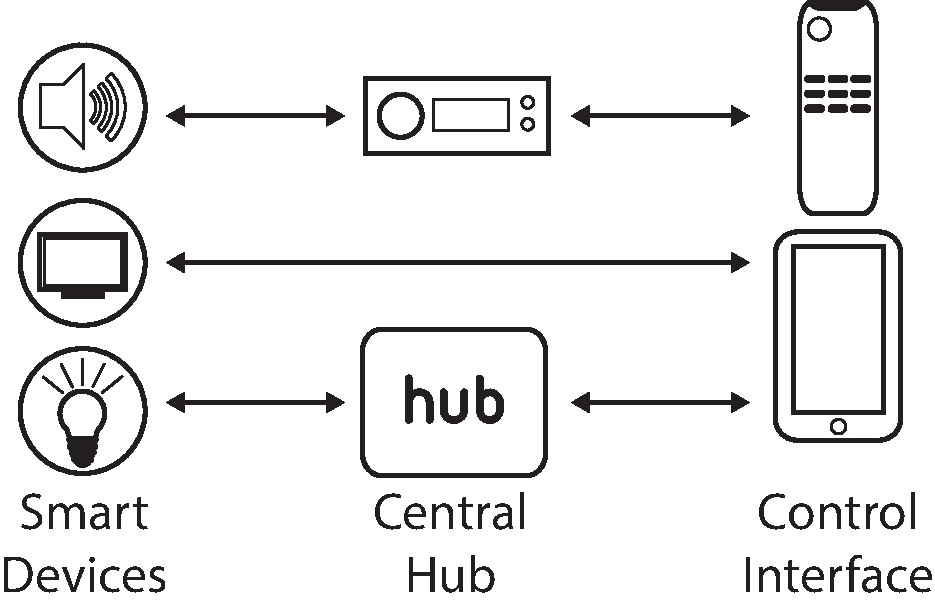
\includegraphics[width=\textwidth -200px]
     {graphics/smarthome-john.pdf}}
     \caption{\label{fig:use-case-1} Illustration of John's use case.}
\end{figure}


\begin{colbox}{Use case: Arthur}
Arthur likes to listen to music when he is at home. He has therefore purchased expensive built-in wireless speakers for every room. The speakers can only be controlled through a \hub~from a \phone. One day Arthur comes home from work and tries to turn on the music, but something is wrong - there is no sound coming from the speakers. After checking both the speakers and the wireless network without results, he discovers that the problem is that the \hub~is broken. He now has to wait for the \hub~to be repaired. This use case is illustrated in \figref{fig:use-case-2}.
0\end{colbox}

\begin{figure}[H]
     \center{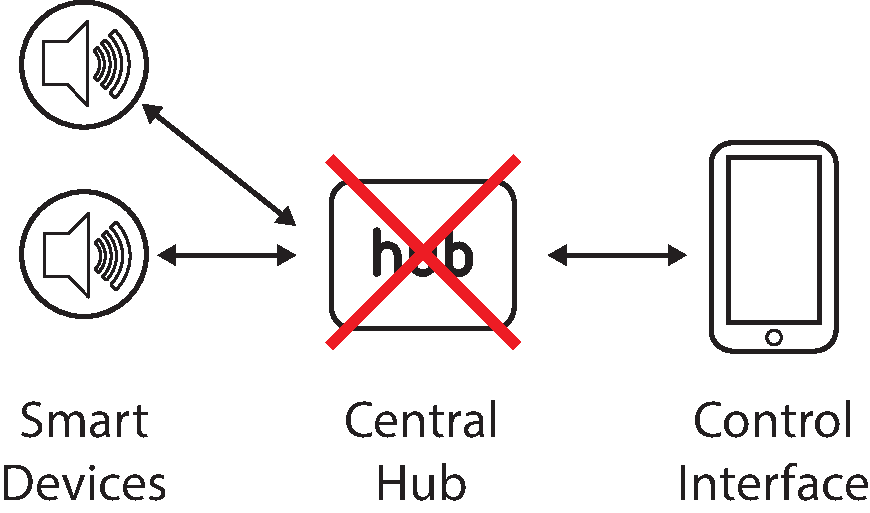
\includegraphics[width=\textwidth -200px]
     {graphics/smarthome-arthur.pdf}}
     \caption{\label{fig:use-case-2} Illustration of Arthur's use case.}
\end{figure}


\begin{colbox}{Use case: Sarah}
Sarah is interested in new technology, and as such she has a Smart Home system. Sarah lives on a farm far away from the city, where she works on the family farm. Unfortunately, Sarah lives in a part of the country where the Internet connection is unstable. Her Smart Home system requires Internet connection to communicate between her devices, where the requests must go through a remote server. This use case is illustrated in \figref{fig:use-case-3}.
\end{colbox}

\begin{figure}[H]
     \center{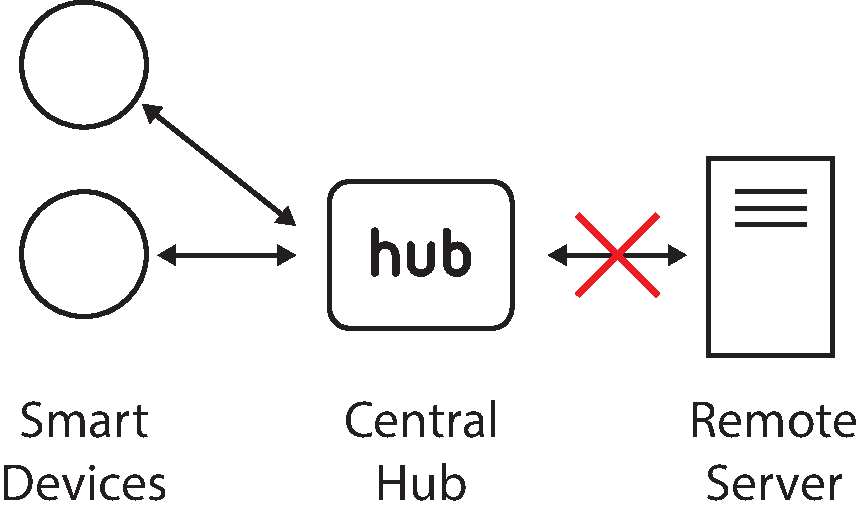
\includegraphics[width=\textwidth -200px]
     {graphics/smarthome-sarah2.pdf}}
     \caption{\label{fig:use-case-3} Illustration of Sarah's use case.}
\end{figure}

\begin{colbox}{Use case: Alice}
Alice lives alone and has a Smart Home system. Usually she is the only one with access to her Smart Home System. One day a new neighbour, Mallory, moved in and asked to borrow Alice Wi-Fi connection for a short period. After some days, the lights and television in Alice's house are turned on at strange times without any interaction from Alice. This use case is illustrated in \figref{fig:use-case-4}.
\end{colbox}

\begin{figure}[H]
     \center{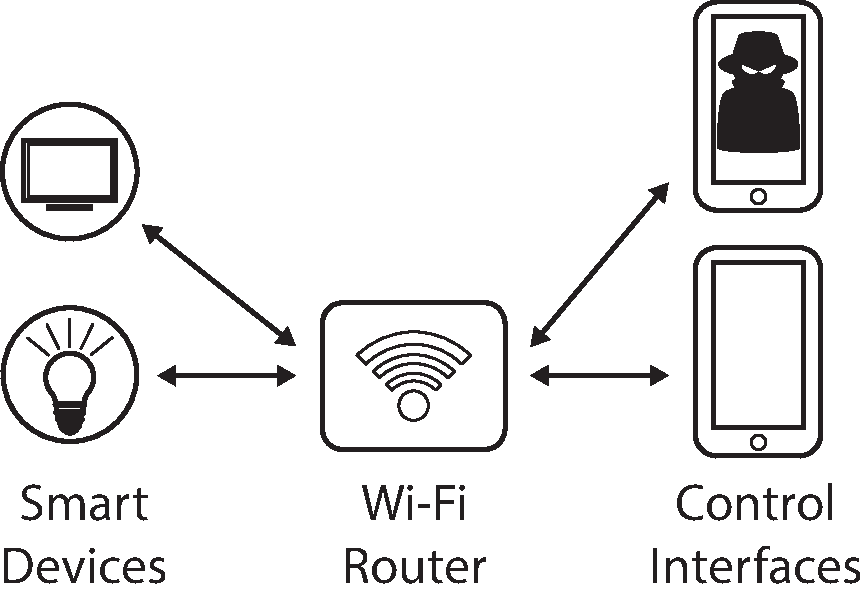
\includegraphics[width=\textwidth -200px]
     {graphics/smarthome-alice.pdf}}
     \caption{\label{fig:use-case-4} Illustration of Alice's use case.}
\end{figure}


These use cases are some of the possible problems that Smart Home owners could have. The four Smart Homes in the use cases suffers from the following issues: no interoperability between manufacturers, centralised around a \hub, requires constant access to remote server, and no user authentication. These problems serve as a base for the further analysis and are referred to through the rest of the report.

\subsection{Smart Home Features} \label{sec:smart-home-features}
When developing a Smart Home system, there are various important aspects to consider. A Smart Home solution should attempt to solve some of the problems occurring in the use cases. Along with the problems found, problems like security, stability, and user-friendliness are also important to consider. The following section are the desired and important properties based on our understanding of the perfect Smart Home system. 

\subsubsection{Stability}
There are two aspects of stability to consider; hardware stability and software stability. \Sdevs~have several external influences which can have unwanted effect on their performance, none of which is preventable with software. The \sdevs~can have an unstable connection to either Wi-Fi or the \hub, they will shut down in case of blackout, and the \hub~can break down. 

Besides the hardware issues, there are also several things that can go wrong on a software level. If the system is not using a \hub~but rather relies on the \phones~being able to connect directly to the \sdevs, a mismatch between the \phones~could occur. Another software instability was found by Raul Rojas. One evening he came home and none of his \sdevs~were working. It turned out that one of his light bulbs had burst and kept reporting it to \hub. This resulted in the light bulb doing a DoS attack on the \hub, which effectively shut down the entire Smart Home~\citep{self-dos-smart-house}.


\subsubsection{Security}
Security is an important aspects to consider. A Smart Home should be secure so that only authorised people can access the Smart Home system. There should also be different levels of access; owners should be able to control the entire system, while guests should only have access rights to the non-sensitive \sdevs. Accessing \sdevs~in a house could potentially expose sensitive data and surveillance media.

Regarding security there are different forms that must be considered. In this project the focus will be on confidentiality, authenticity, and integrity.
\begin{description}
\item[Confidentiality] prevents sensitive information from reaching the wrong people and allowing the right people to access the information.
\item[Authenticity] security of access to devices from people on the same network. Only authorised people should be able to access devices.
\item[Integrity] concerns with keeping the data intact when sent over the network. The data should not be changed by unauthorised people. 
\end{description} 

\subsubsection{Usability}
Setting up a complete Smart Home system can get technical. Ensuring user-friendliness could help expand the market, and improve the user experience. A well designed user interface, or preferred OS compatibility, could also be the deciding factor when choosing the right Smart Home system. This user-friendliness includes both setting up and using the system.

\subsubsection{Interoperability}
Interoperability refers to the ease of connecting additional \sdevs~to the Smart Home system. This is not restricted to \sdevs~from the same manufacturer. As \sdevs~are developed by many different manufacturers it is important to introduce interoperability, a higher level of interoperability could allow easy setup of new \sdevs.

\subsubsection{Feature Contradiction}
These features are all important properties to consider for a Smart Home solution. However it might not be possible to have a high degree of all of these properties as some of them might conflict. Security is, arguably, an important aspect - as no one wants their sensitive data compromised or unauthorised access to their home. This, however, may hurt the usability of the system as it requires management of different access rights.

There are also potential issues with interoperability. It is desirable to be able to connect to any \sdevs, but some devices could possibly have security flaws or other unwanted properties that could both compromise the security and stability of the system.

The stability property in general is intricate. There are multiple areas with potential instability, such as a communicating hub, a Wi-Fi hotspot or the outgoing Internet connection. Attempting to solve these stability issues by cutting corners, changing, or removing some of the precarious spots could potentially give issues regarding the other properties, for instance security or interoperability.  

% Initiating Problem
\section{Initiating Problem} \label{sec:initiating-problem}

Kort forklaring af at der er mange wifi produkter som alle har hver deres app. Kom ind på at SmartHome teknologien.

Også tilføj en del med motivation, hvorfor er der behov for dette og er det en god ide?

% Existing Solutions
\section{Existing Solutions} \label{sec:existing-solutions}

For at få en videre forståelse omkring SmartHome så kigger vi på konkurrenterne.

% Target group
\section{Target Group} \label{sec:target-group}

The existing solutions are primarily targeting upper middle class citizens, as the components and devices needed are quite expensive. Taking into consideration that the technology is rather new and constantly evolving, the pricing is understandable. However there might be people with less money to spend or people who already own different \sdevs, who are also interested in having an automated home.

Another possible target group are handicapped and chronically ill people~\citep{overview-smart-home-environment}. A Smart Home system could drastically improve their quality of life, by giving these people easier access to devices. Some problems they could experience include, reaching switches, bending down to reach devices at floor level, and blind people that cannot change channels etc~\citep{disabled-smart-home}. This could also affect temporary ill people, that for a period of time might be constrained to their beds or the like. If these people could access their house devices through a Smart Home solution, a lot of trouble could be avoided. 

The problem is that a lot of the Smart Home systems only work with their own products and an expensive \hub~is required for the Smart Home system to even work. As such, people may not be able to make such an investment or they may not be able to connect all of their current devices into one system. Overcoming these problems by avoiding a \hub~and increasing the interoperability could make home automation more available and appealing to a broader audience than it currently is. 



% Problem Statement
\section{Problem Statement} \label{sec:problem-statement}

Vi vil lave et SmartHome hvor man selv kan justere hvilke produkter der skal kunne styres fra web tjenesten.

Slut af med problem statement.

% Problem Specification
\section{Problem Delimitation} \label{sec:problem-delimitation}

The Smart Home system developed in this project is a prototype trying to overcome some of the problems found in the use cases from \secref{sec:use-cases}. Due to the length of the project and limited resources, the project does not focus on building a complete Smart Home system.
Instead the focus is to solve the problems found in the use cases. As such, the project has the following limitation: 

\begin{description}
\item[Interoperability] The system will be developed to control smart devices from two different manufactures, to test whether this can be done or not.
\item[Usability] The project will not focus on the usability of the system, which means that no major design decisions or usability evaluation will be conducted.
\item[Decentralisation] The project's primary focus is decentralisation, to see whether or not this can be done.
\item[Security] The system will implement a simple user authentication system. 
\end{description}




\fxnote{fix placement af det her mandag}
A Smart Home Environment is composed of the following components~\citep{overview-smart-home-environment}: 
\begin{itemize}
\item Home Automation System - \Sdevs~in the system
\item Control System - The system that combines and allows manipulation on the \sdevs
\item Home Automation Network - Physical connection and communication protocols used
\end{itemize}

% Design
\chapter{Design} \label{cha:design}

% Implementation
\chapter{Implementation} \label{cha:implementation}





% Frameworks - teknologier der kan bruges til at udvikle sådan et system. 





% Test
\chapter{Test} \label{cha:test}



% Evaluation
\chapter{Evaluation} \label{cha:evaluation}

% Se tilbage på use cases. Fik vi opfyldt deres problemer?



%%%% Kilder %%%%
\begingroup
	\raggedright
	\bibliography{bibliography/literature.bib}
\endgroup
\phantomsection


\addcontentsline{toc}{part}{Appendix}

%%%% Appendiks %%%%
\begingroup
\appendix
\clearforchapter
\phantomsection
% Name \chapter inside the appendices

% Hardware test
%\input{appendix/hardwaretest-appendix.tex}


\endgroup

%%%% Fixme/fxnotes %%%%
\listoffixmes

\end{document}







%%%% Skabelon til et billede %%%%
%\begin{figure}[H]
%     \center{\includegraphics[width=\textwidth]
%     {graphics/Billedenavn.pdf}}
%     \caption{\label{fig:Billedenavn} Billede tekst.}
%\end{figure}

%%%% Skabelon til en lstlisting %%%%
%\begin{lstlisting}[caption= Look at my fancy \lstref{lst:testlst}, label=lst:testlst]
%...
%\end{lstlisting}

%%%% Skabelon til en tabel %%%%
%\begin{table}[H]
%	\centering
%	\ra{1.3}
%   \rowcolors{1}{Gray}{}
%   \begin{tabular}{lcc}
%   \hline  
    
%   Tekst    & Mere tekst    & Endnu mere tekst  \\ \hline  \rowcolor{Gray}
%   Tekst    & Mere tekst    & Endnu mere tekst  \\ 
    %Copy the two lines if more is needed.
    
%   \hline 
%   \end{tabular}
%   \caption{\label{table:TableNameForReferencing} Table tekst.}
%\end{table}